\newpage
\section{ $C^0$ Interior Penalty Method for Biharmonic Equation}
\label{sec:ch1}


% \subsection{Hybrid DG Biharmonic Equation}%
% \label{sub:hybrid_dg_biharmonic_equation}

Let $\Omega \subset   \mathbb{R} ^2$ be a bounded polygonal domain and $\partial \Omega $ be its corresponding boundary. Let the fourth order biharmonic equation have the form,

\begin{equation}
\label{eq:bi_problem}
\begin{split}
    \Delta^2  u  + \gamma u  & = f \quad \text{in } \Omega   \\
    \partial _{n} u & = g_1\left( x \right)  \quad \text{on } \partial \Omega  \\
    \partial _{n} \nabla ^2 u & = g_{2}\left( x \right)  \quad \text{on } \partial \Omega .  \\
\end{split}
.\end{equation}
Here is $\Delta ^2$ the biharmonic operator, also known as the bilaplacian. We will assume for now that $u \in H^{4}\left( \Omega  \right) $, $\gamma $ is nonnegative constants and $f \in L_{2}\left( \Omega  \right) $. We may consider the functions $g_{1}$ and $g_{2}$ as time independent boundary conditions. Such problems as \eqref{eq:bi_problem} are often associated with the Cahn-Hilliard model
\cite{cahnhilliard1957} for phase seperation. As a matter of fact, the major difference is that \eqref{eq:bi_problem}
has no time dependencie. However, depending on how Cahn-Hilliard model is time discretized numerically can
\eqref{eq:bi_problem} naturally arise. I refer to \cite{brenner2012quadratic} for more informastion on this.

Before we start constructing a numerical method, we might want to introduce the basic weak formulation of \eqref{eq:bi_problem}. Now, let the solution space be on the form,
\begin{equation*}
V = \left\{ v \in H^2\left( \Omega  \right) : \partial _{n} v = g_{1}  \text{ on }
\partial \Omega  \right\}.
.\end{equation*}
Consider the weak formulation to solve for a $u \in  V$ such that
\begin{equation}
    \label{eq:bi_weak1}
a\left( u,v \right)_{\Omega } = F(v).\quad \forall v \in
V,
\end{equation}
where the terms are computed as \[
    \begin{split}
a\left( u,v \right)_{\Omega } & = \int_{\Omega }^{} \left( D ^2 u : D ^2 v  +
\gamma u v \right) dx , \\
F\left( v \right)_{\Omega } & = \left( f,v \right)_{\Omega } - \left<g_{2},v \right>_{\partial \Omega } + \left<\nabla g_{1}, \nabla v \right>_{\partial \Omega }.
    \end{split}
\]
We denote $D^2$ as the Hessian matrix operator. In fact, the solution is unique for $\gamma > 0$. However, for $\gamma = 0$ must we assume the solvability condtion,
\begin{equation*}
 \int_{\Omega }^{} f dx = \int_{\partial \Omega }^{} g_{2} ds
.\end{equation*}
This condition easily arise when using the substitution $v=1$ in \eqref{eq:bi_weak1}. To handle this, can we extended the solution space \[
V^{*} = \begin{cases}
    V \quad & \gamma > 0 \\
    \left\{ v \in V: v\left( p_{*} \right)  = 0\right\}, \quad & \gamma = 0
\end{cases}
\]
\todo{ Why is setting test function $v\left( p_{*} \right)  = 0$ on corners interesting?}
where $p_{*}$ is a corner of the polygonal domain $\Omega $.
Thus, the unique solution in $v \in V^{*}$ belongs to $H^{3 }\left( \Omega  \right) $ and we get the follwing
elliptic regularity estimate \cite{gu2012c0},
\begin{equation}
\label{eq:bi_harmonic_ellitpic_regularity}
\left| u \right| _{H^{3 }\left( \Omega  \right) }  \le C_{\Omega } \left( \| f \|_{  L_{2}( \Omega ) }^{  } + ( 1 + \gamma ^{\frac{1}{2}}
) \cdot \| w  \|_{ H^{4}\left( \Omega  \right)  }^{  }    \right), \quad w\in H^{4}\left( \Omega  \right).
\end{equation}
This regularity estimate may be important for further usecases in terms of error analysis.

To solve this numerically do we want to introduce the $C^{0}$ Interior Penalty Method (C0IP), which is a Discontinious Galerkin
method (DG) using $C^{0}$ finite elements. There is several reasons why we want to apply $C^{0}$ instead of the often used
$C^{1}$ finite elements for fourth order problems. First and foremost is the $C^0$ finite elements simpler than
obtaining $C^{1}$ finite elements.  Also, compared to other methods similar to the mixed
finite element method for the problem \eqref{eq:bi_problem}, C0IP has in fact
preserved the symmetric positive definiteness, which means the stability analysis is more straight forward. Finally and most
importantly according to \cite{brenner2012quadratic} can naive use mixed methods of splitting the boundary conditions of
the problem \eqref{eq:bi_problem} produce wrong solutions if $\Omega $ is nonconvex.

\begin{figure}[!h]
\centering
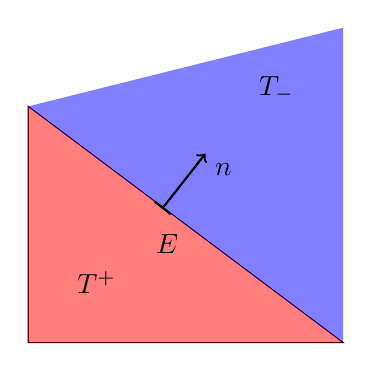
\begin{tikzpicture}[scale=1]
\coordinate (A) at (0,0);
\coordinate (C) at (0,3);
\coordinate (B) at (4,0);
\coordinate (D) at (4,4);
\coordinate (Tm) at (3.5,3.5);
\coordinate (Tp) at (0.5, 0.5);
\coordinate (e) at (1.5, 1.5);
\coordinate (start) at (1.7, 1.7);
\coordinate (end) at (2.25, 2.4);

\draw (A) -- (B) -- (C) -- cycle;
\fill[red, opacity=0.5] (A) -- (B) -- (C);
\fill[blue, opacity=0.5] (B) -- (C) -- (D);
\node[below left] at (Tm) {$T_{-} $ };
\node[above right] at (Tp) {$T^{+}$ };
\node[below right] at (e) {$E$ };

\draw [|->, thick] (start) -- (end);
% \node[above right] at (A) {A };
% \node[below right] at (B) {B};
% \node[above right] at (C) {C };
% \node[below right] at (D) {D};
\node[below right] at (end) {$n$};
\end{tikzpicture}
\caption{Edge $E \in \mathcal{F}_h $ shared by the triangles $T^{+}, T^{-} \in \mathcal{T}_{h} $ and the normal unit vector $n$.  }
    \label{fig:normal}
\end{figure}

Let $w,v \in  H^{4} \left( T  \right) $ and $\mathcal{T}_{h} $ the simplicial triangulation of $\Omega$. Using the same method as in \cite{gu2012c0, brenner2012quadratic} can we
deduce that for every triangle $T \in  \mathcal{T}_{h} $ is \[
    \begin{split}
        \left( \Delta  ^{2} w, v \right) _{T} &= \left< \partial _{n} \nabla ^2 w, v \right>_{\partial T} - \left( \nabla \left( \nabla ^2 w
 \right), \nabla  v  \right)_{T}   \\
 &= \left( D^2w, D^2v \right)_{T} + \left< \partial _{n} \nabla ^2 w, v \right>_{\partial T}  - \left<\partial _{n}
 \nabla w, \nabla v \right>_{\partial T} \\
 &=  \left( D^2 w, D^2 v \right)_{T} - \left<\partial _{nt} w, \partial _{t} v \right>_{\partial T} - \left<\partial
 _{nn} w, \partial _{n} v \right> _{\partial T} +  \left<\partial _{n} \nabla ^2 w, v \right>_{\partial T} \\
    \end{split}
\]
Keep in mind that this result naturally arise when defining $\nabla  = \left( \partial _{n}, \partial _{t} \right) $ such that
\[
\left<\partial _{n} \nabla w, \nabla v \right>_{\partial T} = \left<\partial _{nt} w, \partial _{t} v\right> _{\partial
T} + \left< \partial _{nn} w, \partial _{n} v  \right> _{\partial T} .
\]
 Thus, letting $u,v \in
H^{4}\left( T  \right) $  does this hold ,

\begin{equation}
\label{eq:bi_basic_dg}
\left( \Delta  ^{2} u,v \right) _{T} =  \left( D^2u,D^2v \right) _{T } - \left<\partial _{nt} u, \partial _{t}v
\right>_{\partial T} - \left<\partial _{nn} u, \partial _{n}v \right>_{\partial T} + \left<\partial _{n} \nabla ^2 u,v
\right>_{\partial T}
.\end{equation}

For global continuity, let  $v \in V =  \left\{ v \in H^{1}\left( \Omega  \right): v_{T} \in  H^{4}\left( T \right), \ \forall T \in
\mathcal{T}_{h}    \right\}   \cap C^{0} (
\overline{\Omega }  ) $ and $u \in  H^{4}\left( \Omega  \right) $ such that,

\begin{equation}
\label{eq:bi_basic_dg2}
\left( \Delta  ^{2} u,v \right) _{\Omega } = \sum_{T \in  \mathcal{T} _{h}}^{} \left( D^2u,D^2v \right) _{T } - \left<\partial _{nt} u, \partial _{t}v
\right>_{\partial T} - \left<\partial _{nn} u, \partial _{n}v \right>_{\partial T} + \left<\partial _{n} \nabla ^2 u,v
\right>_{\partial T}
.\end{equation}

However, this can be simplified to

\begin{equation}
\label{eq:bi_basic_dg_full_1}
\begin{split}
\left( \Delta  ^{2} u, v \right) _{\Omega }
=& \sum_{T \in  \mathcal{T} _{h}}^{} \left( D^2u, D^2v \right)_{T}  + \sum_{E \in
\mathcal{F} ^{ext}_{}}^{} \left<\partial _{n} \nabla  ^2 u, v  \right> _{E}
- \left<\partial _{nt} u, \partial _{t} v \right> _{E}+
\left< \partial _{nn} u, \partial _{n} v \right>_{E} + \sum_{E \in \mathcal{F}  ^{int}}^{} \left<\partial _{nn} u , \jump{ \partial _{n} v }
\right>_{E} \\
& = \sum_{T \in  \mathcal{T} _{h}}^{} \left( D^2u, D^2v \right)_{T} + \sum_{E \in
\mathcal{F} ^{ext}_{}}^{} \left<g_{2 }, v  \right> _{E}
+ \left<n g_{2}, \nabla _{n}v \right>_{E} + \left<\partial _{t} g_{1} , \partial _{t}v \right>_{E}
+ \sum_{E \in \mathcal{F}  ^{int}}^{} \left< \partial _{nn} u    , \jump{ \partial_{n} v } \right>_{E}
\end{split}
\end{equation}
Where $\mathcal{F}^{int}_h , \mathcal{F} ^{ext}_{h} \subset \mathcal{F}_{h} $ be the set of interior and exterior facets of the triangulation $\mathcal{T}_{h} $.
Keep in mind that the jump over and edge $E$, visualized in figure \ref{fig:normal},   is defined as $\jump{ a } =    a^{+} - a^{-} $
and similarly will the mean be defined as $\mean{ a  } = \frac{1}{2}(   a^{+}
+ a^{-})$.  The equivalence of \eqref{eq:bi_basic_dg2} and \eqref{eq:bi_basic_dg_full_1} comes from the following argumentation.

\begin{equation*}
    \begin{split}
 \left( \Delta  ^{2} u,v \right) _{\Omega } & =\sum_{T\in \mathcal{T} _{h}}^{} \left( D^2u,D^2v \right) _{T } - \left<\partial _{nt} u, \partial _{t}v
\right>_{\partial T} - \left<\partial _{nn} u, \partial _{n}v \right>_{\partial T} + \left<\partial _{n} \nabla ^2 u,v
\right>_{\partial T} \\
&= \sum_{T\in \mathcal{T} _{h}}^{} \left( D^2u,D^2v \right) _{T } \\
&  \quad + \sum_{E \in \mathcal{F}_{h}^{ext} }^{} \underbrace{\left< \partial _{n} \nabla ^2 u, v  \right>_{E}}_{= \left< g_{2},v \right>_{E} }  -  \underbrace{\left<
\partial _{nt} u, \partial _{t} v \right> _{E}}_{= \left<\partial _{t} g_{1} , \partial _{t}v \right> }  - \underbrace{\left< \partial _{nn} u, \partial _{n} v \right>}_{= \left<n g_{2}, \partial  _{n}v \right>_{E}  }    \\
& \quad  + \sum_{E \in \mathcal{F} _{h}^{int}}^{} \underbrace{\left( \left<\partial _{n^{+}} \nabla ^2 u^{+}
        ,v^{+}\right>_{E}
+ \left<\partial _{n^{-}} \nabla ^2 u^{+} ,v^{-}\right>_{E}  \right)}_{(I)} +
\underbrace{\left( \left<\partial _{n^{+}t} u^{+}, \partial_{t} v^{+} \right>_{E} +  \left<\partial _{n^{-}t} u^{-},
        \partial_{t} v^{-}
\right>_{E}  \right) }_{(II)} +
\underbrace{\left( \left<\partial _{n^{+}n^{+}} u^{+}, v^{+} \right> _{E} + \left<\partial _{n^{-}n^{-}} u^{-}, v^{-}
\right> _{E} \right) }_{(III)}
    \end{split}
.\end{equation*}

Where integration over all interior edges $ \forall E \in \mathcal{F}_{h}^{int}$ is computed in this way:
\begin{equation*}
    \begin{split}
        (I) &  =    \left<\partial _{n^{+}} \nabla ^2 u^{+} ,v^{+}\right>_{E} +
        \left<\partial _{n^{-}} \nabla ^2 u^{+} ,v^{-}\right>_{E} =   \int_{E}^{}
        \jump{ \partial _{n} \nabla ^2 u \cdot v } =
         \int_{E}^{}
         \mean{ \partial _{n} \nabla ^2 u } \underbrace{\jump{ v }}_{= 0}    + \underbrace{\jump{ \partial _{n} \nabla ^2 u
         }}_{= 0}    \mean{ v } = 0 \\
        (II) &  =     \left<\partial _{n^{+}t} u^{+}, \partial_{t} v^{+}
        \right>_{E} +  \left<\partial _{n^{-}t} u^{-}, \partial_{t} v^{-}
\right>_{E}    =   \int_{E}^{}
        \jump{ \partial _{nt} u \cdot  \partial_{t} v } =
         \int_{E}^{}
         \mean{ \partial _{nt} u    } \underbrace{\jump{ \partial_{t} v }  }_{= 0}    + \underbrace{\jump{ \partial
                 _{nt}  u
         }}_{= 0}    \mean{ \partial _{t}v }  = 0\\
        (III) &  =     \left<\partial _{n^{+}n^{+}} u^{+}, \partial_{n^{+}} v^{+} \right>_{E} +  \left<\partial _{n^{-}n^{-}} u^{-}, \partial_{n^{-}} v^{-} \right>_{E}    =    \int_{E}^{} \jump{ \partial _{nn} u \cdot  \partial_{n} v } = \int_{E}^{}
        \mean{ \partial _{nn} u    } \underbrace{\jump{ \partial_{n} v }  }_{\neq 0}    + \underbrace{\jump{ \partial
                 _{nn}  u
         }}_{= 0}    \mean{ \partial _{n}v } =
        \left< \partial _{nn} u    , \jump{ \partial_{n} v } \right>_{E}  \\
    \end{split}
.\end{equation*}

Observe that the cancellations in the term $(I)$ appears of the continuity of $v\in V $ and $u\in H^{4}\left( \Omega  \right) $ which makes the jumps zero. For the second term $(II)$ does the terms become zero cancelled because the tangential derivative at the edge
has no jump. However, The third term $(III)$  is fairly interesting since the discontinuity in normal vector for $v \in V$ is a jump, while the second term is still continious. It can also be raised that $\mean{ \partial _{nn} u } = \partial _{nn} u  $ holds by the continuity of $H^{4}\left( \Omega  \right) $. Anyhow, the definition of jump of should more interesting when we later weakend the continuity of $u$ during discretization.
Hence, \eqref{eq:bi_basic_dg2} and \eqref{eq:bi_basic_dg_full_1} is equivalent.

We can finally start defining the fully discrete formulation. Let the basis be a $\mathcal{P}_{2} $ Lagrange finite element space so,
\[
V_{h} = \left\{ v \in C^{0}\left( \Omega  \right): v_{T} = v | _{T} \in P_{2}\left( T \right), \forall T \in
\mathcal{T}_{h}    \right\}
\]
and
\[
V_{h}^{*} = \begin{cases}
    V_{h} & \text{ if } \gamma > 0 \\
    \left\{ v \in V_{h}: v\left( p_{*}  \right) = 0   \right\} &  \text{ if } \gamma  = 0
\end{cases}
\]
Now, if we choose $u \in V_{h}$ must we take account that the jump is discrete.
 We have now the final C0IP formulation.
The discretized numerical problem is to solve $w_{h} \in V_{h}^{*}$ such that \[
\mathcal{A}\left( w_{h}, v_{h} \right)   = F\left( v_{h} \right), \quad \forall v_{h} \in V_{h}^{*}  .
\]
where
\begin{equation}
\label{eq:C0IP_A_h_1}
\begin{split}
\mathcal{A} \left( w_{h}, v_{h} \right)   =&
  \quad  \left( \gamma w_{h}, v_{h} \right) _{\Omega }\\
&  + \sum_{T \in \mathcal{T} _{h}}^{} \left( D^2 w_{h}, D^2v_{h} \right) _{T} \\
 & +
  \sum_{E \in \mathcal{F}_{h}^{int} }^{}
  \left< \mean{  \partial _{n n} w_{h} }, \jump{ \partial _{n }v_{h}} \right>_{E}  +
 \left< \mean{ \partial _{n n} v_{h} }, \jump{ \partial _{n}w }      \right>_{E}
+ \tau _{E} \left< \jump{ \partial _{n} w_{h}}, \jump{ \partial _{n} v_{h}   }   \right>_{E}
\end{split}
\end{equation}
and
\begin{equation}
\label{eq:C0IP_F_h}
F\left( v_{h} \right)  = \left( f, v_{h} \right) _{\Omega } +  \sum_ {\mathcal{F} ^{ext}_{}}^{} \left<g_{2 }, v_{h}  \right> _{E}
+ \left<n g_{2}, \partial  _{n}v_{h} \right>_{E} + \left<\partial _{t} g_{1} , \partial _{t}v_{h} \right>_{E}
\end{equation}
Notice that the regulation term with $\tau _{E} = \sigma / \left\lvert E \right\rvert $ is to be determined by respectively a global tuning parameter $\sigma >0 $ and edge length $\left\lvert E \right\rvert $. Another key component to the formulation
in \eqref{eq:C0IP_A_h_1} after introduction of $ w_{h}, v_{h} \in V^{*}_{h}$  is that we expanded $\left< \partial _{nn}w, \jump{ \partial _{n} v }  \right>_{E} \to \left< \mean{ \partial _{nn}w_{h} }  , \jump{ \partial _{n} v_{h} }  \right>_{E} $ since we can longer not guarantee a
continious jump. For symmetric purposes we also added $ \left< \mean{ \partial _{nn} v_{h}}  , \jump{ \partial _{n} w_{h} }  \right>_{E} $.

We may introduce the compact notation of \eqref{eq:C0IP_A_h_1}.

\begin{equation}
\label{eq:C0IP_A_h}
\begin{split}
\mathcal{A} \left( w_{h}, v_{h} \right)   =&
  \quad  \left( \gamma w_{h}, v_{h} \right) _{\Omega }\\
&  +  \left( D^2 w_{h}, D^2v_{h} \right) _{\mathcal{T} _{h}} \\
 & +
  \left< \mean{  \partial _{n n} w_{h} }, \jump{ \partial _{n }v_{h}} \right>_{\mathcal{F}_{h}}  +
 \left< \mean{ \partial _{n n} v_{h} }, \jump{ \partial _{n}w }      \right>_{\mathcal{F}_{h}}
+ \tau _{E} \left< \jump{ \partial _{n} w_{h}}, \jump{ \partial _{n} v_{h}   }   \right>_{\mathcal{F}_{h}}
\end{split}
.\end{equation}
% In \cite{gu2012c0} they introduce \[
%             \begin{split}
%     \left( D^2v: D^2w \right)_{T } & = \left<\partial _{nt} v , \partial _{t} w  \right>_{\partial T} + \left< \partial
%     _{nn} v
%     \partial _{n}, w \right>_{\partial T}. \\
%     &= \sum_{i=1}^{3} \partial _{n_{i} t_{i}} v \int_{E_{i}}^{} \partial _{t} w ds +\left< \partial
%     _{nn} v,
%     \partial _{n} w \right>_{\partial T}     \\
%     &=\left< \partial
%     _{nn} v,
%     \partial _{n} w \right>_{\partial T}  \\
%             \end{split}
%     \]
% Using the identity $ab +cd = \frac{1}{2} (a+c)(b+d) + \frac{1}{2}(a-c)(b-d) $  they end up with the equations  \[
%     \sum_{T \in \mathcal{T}_{h}  }^{} \left( D^2v: D^2w \right)_{T }  =
%     - \sum_{E \in \mathcal{F} ^{int}}^{}  \mean{ \partial _{n n} v  } \jump{ \partial _{n} w } - \jump{
%     \partial _{n n} v}  \mean{ \partial _{n} w }
% \]

\subsubsection{HC0IP Method copied from NGSolve}%
\label{ssub:hc0ip_method_from_ngsolve}

We consider the Kirchhoff plate equation: Find $w \in H^2$, such that

$$
\int \nabla^2 w : \nabla^2 v = \int f v
$$

A conforming method requires $C^1$ continuous finite elements. But there is no good option available, and thus there is no $H^2$ conforming finite element space in NGSolve.

$$
\sum_T \nabla^2 w : \nabla^2 v
- \int_{E} \{\nabla^2 w\}_{nn} \, [\partial_n v]
- \int_{E} \{\nabla^2 v\}_{nn} \, [\partial_n w] + \alpha \int_E  [\partial_n w]  [\partial_n v]
$$

[Baker 77, Brenner Gudi Sung, 2010]

We consider its hybrid DG version, where the normal derivative is a new, facet-based variable:


$$
\sum_T \nabla^2 w : \nabla^2 v
- \int_{\partial T} (\nabla^2 w)_{nn} \, (\partial_n v - \widehat{v_n})
- \int_{\partial T} (\nabla^2 v)_{nn} \, (\partial_n w - \widehat{w_n}) + \alpha \int_E (\partial_n v - \widehat{v_n}) (\partial_n w - \widehat{w_n})
$$
% Anyhow,
% let us first define the Hilbert space of the discrete solution \[
% \begin{split}
%     H^{1}\left( \mathcal{T}_{h}  \right)  & = \left\{ v \in L_{2} \left( \Omega  \right) : v  \mid _{T} \in H^{1} \left( T
%     \right) \forall T \in \mathcal{T}_{h}    \right\} \\
%     V &=  \left\{ v \in H^2\left( \Omega  \right) : \partial _{n} v = 0 \text{ and } \partial _{n} \nabla ^2 v = 0 \text{ on } \partial \Omega  \right\} \\
% \end{split}
% \]
% \todo[inline]{ Probably need to work more on this argumentation }

% Let us now define $u,v \in V$.

% \subsubsection{HDG Method}%
% \label{ssub:dg_method}
% Let us now define our workspace using the spaces

%  \[
% \begin{split}
%     V &=  \left\{ \left( u, u_{F}  \right): u \in H^{4}\left( \mathcal{T} _{h} \right) \cap H^{1}\left( \Omega  \right)   \right\} \\
%     V_{h} &=  \left\{ \left( u, u_{F}  \right) : u \in \mathcal{P} ^{k}\left( T \right) \forall T \in  \mathcal{T} ,
%     u_{F} \in \mathcal{P} ^{k}\left( E \right) \forall E \in  \mathcal{F}_{h}    \right\} \\
% \end{split}
% \]

% and the ones including the null drichlet conditions \[
% \begin{split}
%     V_{0} &= \left\{ \left( u, u_{F} \right) \in  V : \quad u =0, u_{F} = 0 \text{ on } \partial \Omega   \right\}, \\
%     V_{0,h} &= \left\{ \left( u, u_{F} \right) \in  V_{h} : \quad u =0, u_{F} = 0 \text{ on } \partial \Omega   \right\}
%    . \\
% \end{split}
% \]
% Let $\left( u, u_{F} \right) \in  V $\[
%     \begin{split}
% \sum_{T}^{} \left( \nabla ^{4} u,v \right) & = \sum_{T}^{} \left( \nabla ^{3} u, \nabla  v \right)_{T} + \left<\partial _{n}
% \nabla ^2 u, v \right>_{\partial \Omega } \\
% &= \sum_{T}^{} \left( \nabla ^2 u, \nabla ^2 v \right)_{T} - \left<\partial _{n} \nabla u, \nabla v \right>_{\partial T}
% + \left< \partial _{n} \nabla ^2 u, v \right> _{\partial T}\\
%     \end{split}
% \]




